%%%%%%%%%%%%%%%%%%%%%%%%%%%%%%%%%%%%%%%%%
% KOMA-Script Presentation
% LaTeX Template
%%%%%%%%%%%%%%%%%%%%%%%%%%%%%%%%%%%%%%%%%

%----------------------------------------------------------------------------------------
%	PACKAGES AND OTHER DOCUMENT CONFIGURATIONS
%----------------------------------------------------------------------------------------

\documentclass[
paper=128mm:96mm, % The same paper size as used in the beamer class
fontsize=11pt, % Font size
pagesize, % Write page size to dvi or pdf
parskip=half-, % Paragraphs separated by half a line
]{scrartcl} % KOMA script (article)

\linespread{1.12} % Increase line spacing for readability

%------------------------------------------------
% Colors


\usepackage[dvipsnames]{xcolor} % Required for custom colors
% Define a few colors for making text stand out within the presentation
\definecolor{mygreen}{RGB}{0,128,128}
\definecolor{myblue}{RGB}{0,0,128}
\definecolor{mybrown}{RGB}{194,164,113}
\definecolor{myred}{RGB}{128,0,0}
% Use these colors within the presentation by enclosing text in the commands below
\newcommand*{\mygreen}[1]{\textcolor{mygreen}{#1}}
\newcommand*{\myblue}[1]{\textcolor{myblue}{#1}}
\newcommand*{\mybrown}[1]{\textcolor{mybrown}{#1}}
\newcommand*{\myred}[1]{\textcolor{myred}{#1}}
%------------------------------------------------

%------------------------------------------------
% Margins
\usepackage[ % Page margins settings
includeheadfoot,
top=3.5mm,
bottom=3.5mm,
left=5.5mm,
right=5.5mm,
headsep=6.5mm,
footskip=8.5mm
]{geometry}
%------------------------------------------------

%------------------------------------------------
% Fonts
\usepackage[T1]{fontenc}	 % For correct hyphenation and T1 encoding
\usepackage{lmodern} % Default font: latin modern font
%\usepackage{fourier} % Alternative font: utopia
%\usepackage{charter} % Alternative font: low-resolution roman font
\renewcommand{\familydefault}{\sfdefault} % Sans serif - this may need to be commented to see the alternative fonts
%------------------------------------------------

%------------------------------------------------
% Various required packages
\usepackage{amsthm} % Required for theorem environments
\usepackage{amsmath}
\usepackage{latexsym}
\usepackage{amsfonts}
\usepackage{bm} % Required for bold math symbols (used in the footer of the slides)
\usepackage{graphicx} % Required for including images in figures
\usepackage{tikz} % Required for colored boxes
\usepackage{booktabs} % Required for horizontal rules in tables
\usepackage{multicol} % Required for creating multiple columns in slides
\usepackage{lastpage} % For printing the total number of pages at the bottom of each slide
\usepackage[english]{babel} % Document language - required for customizing section titles
\usepackage{microtype} % Better typography
\usepackage{tocstyle} % Required for customizing the table of contents
\usepackage[utf8]{inputenc}

%------------------------------------------------

%------------------------------------------------
% Slide layout configuration
\usepackage{scrpage2} % Required for customization of the header and footer
\pagestyle{scrheadings} % Activates the pagestyle from scrpage2 for custom headers and footers
\clearscrheadfoot % Remove the default header and footer
\setkomafont{pageheadfoot}{\normalfont\color{black}\sffamily} % Font settings for the header and footer

% Sets vertical centering of slide contents with increased space between paragraphs/lists
\makeatletter
\renewcommand*{\@textbottom}{\vskip \z@ \@plus 1fil}
\newcommand*{\@texttop}{\vskip \z@ \@plus .5fil}
\addtolength{\parskip}{\z@\@plus .25fil}
\makeatother

% Remove page numbers and the dots leading to them from the outline slide
\makeatletter
\newtocstyle[noonewithdot]{nodotnopagenumber}{\settocfeature{pagenumberbox}{\@gobble}}
\makeatother
\usetocstyle{nodotnopagenumber}

\AtBeginDocument{\renewcaptionname{english}{\contentsname}{\Large Content}} % Change the name of the table of contents
%------------------------------------------------

%------------------------------------------------
% Header configuration - if you don't want a header remove this block
\ihead{
\hspace{-2mm}
\begin{tikzpicture}[remember picture,overlay]
\node [xshift=\paperwidth/2,yshift=-\headheight] (mybar) at (current page.north west)[rectangle,fill,inner sep=0pt,minimum width=\paperwidth,minimum height=2\headheight,top color=mygreen!64,bottom color=mygreen]{}; % Colored bar
\node[below of=mybar,yshift=3.3mm,rectangle,shade,inner sep=0pt,minimum width=128mm,minimum height =1.5mm,top color=black!50,bottom color=white]{}; % Shadow under the colored bar
shadow
\end{tikzpicture}
\color{white}\runninghead} % Header text defined by the \runninghead command below and colored white for contrast
%------------------------------------------------

%------------------------------------------------
% Footer configuration
\setlength{\footheight}{8mm} % Height of the footer
\addtokomafont{pagefoot}{\footnotesize} % Small font size for the footnote

\ifoot{% Left side
\hspace{-2mm}
\begin{tikzpicture}[remember picture,overlay]
\node [xshift=\paperwidth/2,yshift=\footheight] at (current page.south west)[rectangle,fill,inner sep=0pt,minimum width=\paperwidth,minimum height=3pt,top color=mygreen,bottom color=mygreen]{}; % Green bar
\end{tikzpicture}
\myauthor\ \raisebox{0.2mm}{$\bm{\vert}$}\ \myuni % Left side text
}

\ofoot[\pagemark/\pageref{LastPage}\hspace{-2mm}]{\pagemark/\pageref{LastPage}\hspace{-2mm}} % Right side
%------------------------------------------------

%------------------------------------------------
% Section spacing - deeper section titles are given less space due to lesser importance
\usepackage{titlesec} % Required for customizing section spacing
\titlespacing{\section}{0mm}{0mm}{0mm} % Lengths are: left, before, after
\titlespacing{\subsection}{0mm}{0mm}{-1mm} % Lengths are: left, before, after
\titlespacing{\subsubsection}{0mm}{0mm}{-2mm} % Lengths are: left, before, after
\setcounter{secnumdepth}{0} % How deep sections are numbered, set to no numbering by default - change to 1 for numbering sections, 2 for numbering sections and subsections, etc
%------------------------------------------------

%------------------------------------------------
% Theorem style
\newtheoremstyle{mythmstyle} % Defines a new theorem style used in this template
{0.5em} % Space above
{0.5em} % Space below
{} % Body font
{} % Indent amount
{\sffamily\bfseries} % Head font
{} % Punctuation after head
{\newline} % Space after head
{\thmname{#1}\ \thmnote{(#3)}} % Head spec
	
\theoremstyle{mythmstyle} % Change the default style of the theorem to the one defined above
\newtheorem{theorem}{Theorem}[section] % Label for theorems
\newtheorem{lemma}[theorem]{Lemma}
\newtheorem{remark}[theorem]{Remark} % Label for remarks
\newtheorem{algorithm}[theorem]{Algorithm} % Label for algorithms
\makeatletter % Correct qed adjustment
%------------------------------------------------

%------------------------------------------------
% The code for the box which can be used to highlight an element of a slide (such as a theorem)
\newcommand*{\mybox}[2]{ % The box takes two arguments: width and content
\par\noindent
\begin{tikzpicture}[mynodestyle/.style={rectangle,draw=mygreen,thick,inner sep=2mm,text justified,top color=white,bottom color=white,above}]\node[mynodestyle,at={(0.5*#1+2mm+0.4pt,0)}]{ % Box formatting
\begin{minipage}[t]{#1}
#2
\end{minipage}
};
\end{tikzpicture}
\par\vspace{-1.3em}}
%------------------------------------------------

%----------------------------------------------------------------------------------------
%	PRESENTATION INFORMATION
%----------------------------------------------------------------------------------------

\newcommand*{\mytitle}{The Vectorial Deffuant Model} % Title
\newcommand*{\runninghead}{Vectorial Deffuant Model } % Running head displayed on almost all slides
\newcommand*{\myauthor}{Alexander Mendelsohn} % Presenters name(s)
\newcommand*{\mydate}{04 July 2016} % Presentation date
\newcommand*{\myuni}{LMU Faculty of Mathematics} % University or department

%----------------------------------------------------------------------------------------

\begin{document}

%----------------------------------------------------------------------------------------
%	TITLE SLIDE
%----------------------------------------------------------------------------------------

% Title slide - you may have to tweak a few of the numbers if you wish to make changes to the layout
\thispagestyle{empty} % No slide header and footer
\begin{tikzpicture}[remember picture,overlay] % Background box
\node [xshift=\paperwidth/2,yshift=\paperheight/2] at (current page.south west)[rectangle,fill,inner sep=0pt,minimum width=\paperwidth,minimum height=\paperheight/3,top color=mygreen,bottom color=mygreen]{}; % Change the height of the box, its colors and position on the page here
\end{tikzpicture}
% Text within the box
\begin{flushright}
\vspace{0.6cm}
\color{white}\sffamily
{\bfseries\Large\mytitle\par} % Title
\vspace{0.5cm}
\normalsize
\myauthor\par % Author name
\mydate\par % Date
\vfill
\end{flushright}

\clearpage

%----------------------------------------------------------------------------------------
%	TABLE OF CONTENTS
%----------------------------------------------------------------------------------------

\thispagestyle{empty} % No slide header and footer
\scriptsize\tableofcontents % Change the font size and print the table of contents - it may be useful to shrink the font size further if the presentation is full of sections
% To exclude sections/subsections from the table of contents, put an asterisk after \(sub)section like so: \subsection*{Results}

\clearpage

%----------------------------------------------------------------------------------------
%	PRESENTATION SLIDES
%----------------------------------------------------------------------------------------

\section{The Standard Voter Model}

\begin{itemize}
\item A spin system (or interacting particle system) is a Feller process on the set $\{0,1\}^V$, where $V$ is a graph such as the $\mathbb{Z}^d$-lattice, and individual transitions involve one site only. 
\item In the standard voter model on $\mathbb{Z}^d$ we can think of each site being occupied by a person, who is either in favour or against a certain issue or candidate.
\begin{equation}
\eta_t: \mathbb{Z}^d \longrightarrow \{0,1\}, t \in \left[ 0, \infty \right) 
\end{equation}
\item At an exponentially distributed time each agent randomly picks one of her neighbours and sets her opinion equal to that of the neighnour.
\item The voter model is defined by the probability generator:
\begin{equation}
Lf(\eta) = \sum_{x \in \mathbb{Z}^d} \frac{1}{2d} \sum_{u \sim x}\left[ f(\eta_{x,u})-f(\eta)\right] 
\end{equation}
\item $\eta_{x,u}$ denotes the configuration obtained from $\eta$ by setting the configuration at $x \in \mathbb{Z}^d$ equal to the configuration at $u \in \mathbb{Z}^d$ and leaving all the other sites unchanged.
\item Where $f$ is continuous, real-valued and $\vert\vert\vert f \vert\vert\vert := \sum_{x,u}sup_{\eta}\vert f(\eta_{x,u})-f(\eta)\vert < \infty$
\end{itemize}
\clearpage
\begin{figure}[!tbp]
  \centering
  \begin{minipage}[b]{0.4\textwidth}
    
\includegraphics[width=\textwidth]{c:/users/alexander/graphics/voterModelinit.PNG}
    \caption{Voter Model, initial configuration}
  \end{minipage}
  \hfill
  \begin{minipage}[b]{0.4\textwidth}
    
\includegraphics[width=\textwidth]{c:/users/alexander/graphics/voterModel.PNG}
    \caption{Voter model after 30K successful interactions}
  \end{minipage}
\end{figure}
\clearpage

\clearpage

\section{The vectorial Deffuant Model}

\begin{itemize}
\item The vectorial Deffuant model extends in the voter model with a state space $\{0,1\}^F$,$F \in \mathbb{N}$ denotes the number of \textbf{features}, and incorporates homophily (with an interaction threshold).
\begin{equation}
\eta_t : \mathbb{Z}^d \longrightarrow \{0,1\}^F
\end{equation}
\item The state space is a hypercube equipped with the Hamming distance 
\begin{equation}
H: \{0,1\}^F\times \{0,1\}^F \rightarrow \mathbb{N}, \: H(u,v):= \vert \{ i: u_{i} \neq v_{i} \} \vert
\end{equation}
\item $\theta \in \{0,1,...,F\}$ is called the \textbf{threshold}.
\item  Each individual picks a random neighbour at rate one and updates
her configuration by moving one unit towards this neighbour along a random direction in the hypercube unless they differ in more than $\theta$ features or both neighbours already agree.
\item Formally the probability generator is given by:
\begin{equation}
\begin{split}
Lf(\eta) = & \sum_{x} {\vert \{y:y \sim x\} \vert}^{-1} \sum_{y \sim x} {\vert \Omega(x,y,\eta) \vert}^{-1} \\ 
& \sum_{u \in \Omega(x,y,\eta)} 1 _{\{ 1 \leq H(\eta(x),\eta(y)) \leq \theta \}} 
[ f(\eta_{x,u})-f(\eta)]
\end{split}
\end{equation}
where $\Omega(x,y,\eta) := \{u \in \{0,1\}^F: H(u,\eta(y)) = H(\eta(x),\eta(y))-1\}$
\item The system is started from a product measure where 
$$ P(\tilde{\eta}_0(x,i)=1)=p, \: 1 \leq i \leq F \text{ and } \forall x\in \mathbb{Z}$$
\end{itemize}

\begin{figure}[!tbp]
  \centering
  \begin{minipage}[b]{0.4\textwidth}
    
\includegraphics[width=\textwidth]{c:/users/alexander/graphics/vDF3T1init.PNG}
    \caption{Initial configuration: F=3, $\theta=1$, $100\times 100$ torus}
  \end{minipage}
  \hfill
  \begin{minipage}[b]{0.4\textwidth}
    
\includegraphics[width=\textwidth]{c:/users/alexander/graphics/vDF3theta1.PNG}
    \caption{100 million successful interactions later}
  \end{minipage}
\end{figure}

\clearpage 

\subsection{Flux, Fixation and Clustering}

\begin{itemize}
\item \textbf{Fluctuation} occurs whenever 
\begin{equation}
P(\eta_t(x) \neq \eta_s(x)\text{ for some } t>s ) = 1 \: \forall x\in V \: \forall s>0
\end{equation} 
\item \textbf{Fixation} occurs if there exists a configuration $\eta_{\infty}$ such that 
\begin{equation}
P(\eta_t(x) = \eta_{\infty} \text{ eventually in } t) = 1 \: \forall x\in V
\end{equation}
i.e. the attributes of each individual is only updated a finite number of times, and a coexistence of different configurations persists. \
\item \textbf{Clustering} occurs if
\begin{equation}
\lim_{t \rightarrow \infty} P(\eta_t(x) = \eta_{t}(x)) = 1 \: \forall x\in V
\end{equation}
i.e. there is a convergence to global consensus. \\
\end{itemize}

\clearpage 

\subsection{Coupling with Annihilating Random Walks}

\begin{itemize}
\item When $d=1$ it is useful to visualise the vec. Deffuant model in terms of a collection of annihilating random walks.
\item We consider the edge between two nearest neighbours $x \sim y \in \mathbb{Z}$ as a space occupied by particles on F levels. A particle at level $i$ on the edge $e=xy$ represents a disagreement between x and y on the Feature $i$.
\begin{figure}[h]
\centering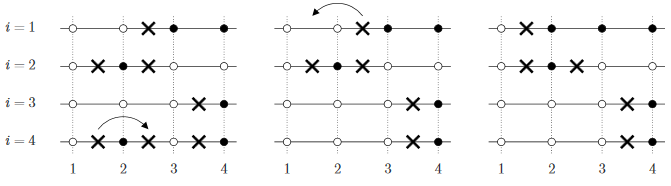
\includegraphics[width=0.7\linewidth]{c:/users/alexander/graphics/annihilatingParticles.PNG}
\caption{\cite{ClustCoex}}
\end{figure}
\item Let $\tilde{\eta_t}: V \times \{1,2,...,F\} \rightarrow \{0,1\} \text{ where } \tilde{\eta_t}(x,i) := \text{ ith coordinate of } \eta_t(x)$.
Then the process corresponding to disagreements is defined by 
$$\xi_t(e,i):= 1_{\{\tilde{\eta_t}(x,i) \neq \tilde{\eta_t}(y,i)\}}$$
where $e=xy$ an edge. $\xi_t$ corresponds to a system of F symmetric annihilating random walks (\textbf{non-independent}).
\item  Extinction of particles is equivalent to a clustering of the system.$$\zeta_t(e):=\xi_t(e,1)+\xi_t(e,2)+...+\xi_t(e,F)= H(\eta_t(x),\eta_t(y))$$
\item An edge will be referred to as a \underline{blockade} if more than $\theta$ particles are on the edge and as an \underline{active edge} if at most $\theta$ particles are on the edge.

\end{itemize}

\clearpage 

\subsection{Graphical Representation}
\begin{itemize}
\item We define a graphical representation for the vec. Deff. model which identifies the system with a percolation structure. The annihilating random walks and the dual process can be constructed from the graphical representation with a standard argument due to Harris (1972). \\

\begin{figure}[h]
\centering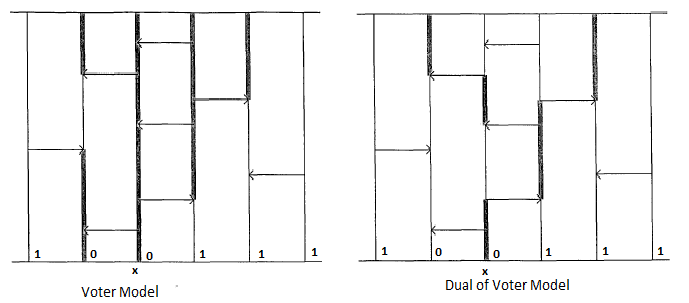
\includegraphics[width=0.76\linewidth]{c:/users/alexander/graphics/graphRepresentation.PNG}
\end{figure}

\clearpage

\item We basically construct F voter models - a graphical representation for each feature with the difference that each path can be active or inactive according to threshold constraints.
\end{itemize}

Let $(x,y,i)\in V  \times V \times \{1,2,...,F\}$ where $x \sim y$
\begin{itemize}
\item we let $(N_{x,y,i}:t \geq 0)$ be a collection of rate one Poisson process
\item we let $T_{x,y,i}(n)$ denote the nth arrival time: $T_{x,y,i}(n):= \inf\{t:N_{x,y,i}=n\}$
\item we let $(B_{x,y,i}(n):n \geq 1)$ be a collection of independent Bernoulli random variables with
\begin{equation}
P(B_{x,y,i}(n)=+1)=P(B_{x,y,i}(n)=-1)=1/2
\end{equation}
\item we let $(U_{x,y,i}(n): n \geq 1)$ be collection of independent Uniform(0,1) random variables.
\end{itemize}
At each time $t:=T_{x,y,i}(n)$ an arrow is drawn from x to y with label $i$, $x\longrightarrow y$ if $B_{x,y,i}(n)=+1$ and from y to x if $B_{x,y,i}(n)=-1$. \\

The arrow $x\longrightarrow y$ is active if
\begin{equation}
\xi_{t-}(e,i)= 1 \text{ and } U_{x,y,i}(n) \leq r(\zeta_{t-}(e)) \text{ where } e=xy
\end{equation}
where 
$$ r(m) := \left\{\begin{array}{cl} m^{-1}, & \mbox{if } 0<m \leq \theta\\ 0, & \mbox{if}\ \theta < m \leq F \end{array}\right.$$

\clearpage

We say there is an active-$i$-path from $(z,s)$ to $(x,t)$, denoted $(z,s) \rightsquigarrow^{i} (x,t)$, whenever there are sequences of times and vertices
$$ s_0 =s<s_1<...<s_{n+1}=t \text{ and } x_0=z, x_1, ...,x_n=x$$
such the following conditions hold:
\begin{itemize}
\item for $j= 1,2,...,n$, there is an active-$i$-arrow $x_{j-1} \longrightarrow x_j$ at time $s_j$, and 
\item for $j= 1,2,...,n$, there is no active-$i$-arrow pointing at $\{x_j\} \times (s_j, s_{j+1})$
\end{itemize}
and there is a \textit{generalized active path} from $(z,s)$ to $(x,t)$, denoted $(z,s) \rightsquigarrow (x,t)$, if 
\begin{itemize}
\item for $j=1,2,...,n$, there is an active arrow $x_{j-1} \longrightarrow x_j$ at time $s_j$
\end{itemize}
\clearpage 

\section{Clustering of the one-dim. 2-Feature vec. Deffuant Model}

\ihead{
\hspace{-2mm}
\begin{tikzpicture}[remember picture,overlay]
\node [xshift=\paperwidth/2,yshift=-\headheight] (mybar) at (current page.north west)[rectangle,fill,inner sep=0pt,minimum width=\paperwidth,minimum height=2\headheight,top color=mygreen!64,bottom color=mygreen]{}; % Colored bar
\node[below of=mybar,yshift=3.3mm,rectangle,shade,inner sep=0pt,minimum width=128mm,minimum height =1.5mm,top color=black!50,bottom color=white]{}; % Shadow under the colored bar
shadow
\end{tikzpicture}
\color{white}2 Features, Threshold 1}

\begin{enumerate}
\item We define a coupling of the 2-Feature vec. Deffuant model to the standard voter model by defining the process:
\begin{equation}
\begin{split}
&\rho_t(x) :=  \vert \tilde{\eta}_{t}(x,1)-\tilde{\eta}_{t}(x,2) \vert \text{ for } x \in \mathbb{Z}^d  \\
&A_1 := \{(0,1),(1,0)\} \longmapsto 1 \\
&A_0 := \{(1,1),(0,0)\} \longmapsto 0
\end{split}
\end{equation}
\item We prove that the voter model fluctuates on $\mathbb{Z}$.
\item The expected number of particles per edge
$$ u(t) := E(\zeta_t(e)) = P(\zeta_t(e)=1)+2P(\zeta_t(e)=2)$$
is independent of edge $e$ due to translation invariance of the initial configuration and symmetric evolution rules.
\item $u(t)$ is non-increasing in time, $\lim_{t \rightarrow \infty} u(t)$ exists almost surely.
\item Let $e=(x)(x+1)$ and $\zeta_t(e)>0$. Then the edge $e$ is either a blockade or an active edge:
\begin{itemize}
\item if $e$ is a blockade it follows from the fluctuation of the voter model $ \tau := \inf \{ s>t: \zeta_s(e) \neq 2 \} = \inf \{ s>t: \rho_s(x) \neq \rho_s(x+1) \} < \infty \text{ a.s.} $. i.e. the blockade is broken in finite time.
\item if $e$ is a live edge, it follows from the recurrence of 1 dimensional symmetric random walks that the active particle at $e$ eventually hits another particle and annihilates or forms a blockade.
\end{itemize}
\item $u(t)$ is strictly decreasing. Particles go extinct almost surely. 

\end{enumerate}

 \clearpage
 
\section{Fixation in the one-dimensional vec. Deff. Model}

\ihead{
\hspace{-2mm}
\begin{tikzpicture}[remember picture,overlay]
\node [xshift=\paperwidth/2,yshift=-\headheight] (mybar) at (current page.north west)[rectangle,fill,inner sep=0pt,minimum width=\paperwidth,minimum height=2\headheight,top color=mygreen!64,bottom color=mygreen]{}; % Colored bar
\node[below of=mybar,yshift=3.3mm,rectangle,shade,inner sep=0pt,minimum width=128mm,minimum height =1.5mm,top color=black!50,bottom color=white]{}; % Shadow under the colored bar
shadow
\end{tikzpicture}
\color{white}Fixation in one-dimension}

We derive a sufficient condition for the fixation of the one-dimensional vec. Deff. Model starting from a product measure. \\
The following Lemma was first proven for cyclic particle systems in \cite{Griffeath89} and more recently extended to the vec. Deff. Model in \cite{ClustCoex}.
\mybox{0.9\textwidth}{
For all $(z,i) \in \mathbb{Z}\times \{ 1,2,...,F \}$, let
\begin{equation}
T(z,i) := \inf \{ t: (z,0) \rightsquigarrow^i (0,t)\}
\end{equation}
Then the vec. Deff. Model fixates whenever
\begin{equation}
\lim_{N \rightarrow \infty} P(T(z,i)< \infty \text{ for some } z<-N \text{ and } i=1,2,...,F) = 0
\end{equation}
}

\clearpage
\subsection{The contribution variable}

"[...] construct a random interval such that all the blockades initially in the interval must have been destroyed by either active particles initially in in this interval or active particles that result from the the destruction of these blockades." \cite[p. 552]{ClustCoex}
\begin{equation}
H_N := \{ T(z,i) < \infty: \text{ for some }z< -N \text{ and some } i=1,2,...,F  \}
\end{equation}
For $T_N:= \inf \{ T(z,i): z < -N \text{ and } i=1,2,...,F\}$  
\begin{equation}
H_N = \{ T_N < \infty \}
\end{equation}

Conditional on the event $H_N$ let $z^*$ be s.t. $T(z^*,i)=T_N$ and let 
\begin{equation}
\begin{split}
z_- & := \min \{ z \in \mathbb{Z}: (z,0) \rightsquigarrow (0,T_N) \} \leq z^* < -N \\
z_+ & := \max \{ z \in \mathbb{Z}: (z,0) \rightsquigarrow (0,S) \text{ for some } S<T_N \} \geq 0
\end{split}
\end{equation}
where $\rightsquigarrow$ now denotes a generalized active path. And let $I_N:= (z_-, z_+)$.\
The contribution variable is defined
\begin{equation}
\begin{split}
&cont: E(\mathbb{Z}) \rightarrow \mathbb{Z}\\
&\text{e \textbf{blockade}}\\
cont(e)&:= \#\{\text{active particles that either annihilate or become frozen as a result} \\
 & \text{of a jump onto $e$ before $e$ becomes a live edge } \} -  \\
 & \#\{ \text{particles initially at $e$ that ever become active} \} \\
&\text{e \textbf{active}}\\
cont(e)&:= \#\{\text{active particles that either annihilate or become frozen as a result} \\
 & \text{of a jump onto $e$ before the first jump of an active particles initially at $e$} \}   \\
 & - \#\{\text{particles initially at $e$} \}
\end{split}
\end{equation}

It follows by definition of $I_N$
\begin{equation}
\begin{split}
& H_N = \{T_N < \infty \} \subseteq \{ \underset{e \in I_N}{\sum}cont(e) \leq 0 \} \\
& \Rightarrow \{ \underset{e \in I_N}{\sum}cont(e) > 0  \} \subseteq \{ T_N= \infty \}
\end{split}
\end{equation}
\clearpage

\subsection{The weight function}

The weight function, as it is named in \cite{ClustCoex} is an explicit random function $\phi: E(\mathbb{Z}) \rightarrow \mathbb{Z}^{\Omega}$ defined to be stochastically smaller that the contribution. So that $\{E(\phi(e))> 0\} \subseteq \{ T_N= \infty \} $ holds for any $e \in E(\mathbb{Z})$.\\
The first jump of an active particle onto a blockade is equally likely to occur at each level and results in
\begin{itemize}
\item an annihilating event with probability $j/F$
\item a blockade increase - extra particle on the edge - with probability $1-j/F$
\end{itemize}
We define the weight function:
\begin{equation}
\begin{split}
&\phi: E( \mathbb{Z} )\rightarrow \mathbb{Z}^{\Omega} \\
&\phi(e):= \left\{\begin{array}{cl} -j, & \mbox{ if } \zeta_0(e)=j \leq \theta \\ 
j + 2(X_{e,j}-\theta), & \mbox{ if } \zeta_0(e)=j > \theta \end{array}\right.
\end{split}
\end{equation}
where $X_{e,j} := Bernoulli(1-j/F)$ and $(X_{e,j})_{e \in E(\mathbb{Z}), 1\leq j \leq F}$ independent.
\clearpage

\mybox{0.8\textwidth}{ % Example of encapsulating text in a colored box
\begin{lemma}
For all $\epsilon>0$, there exists constants $c_6>0$,$C_0>0$ (depending on $F$) such that
$$P((\sum_{e\in (-N,0)}\phi(e)-NE\phi(e)) \not\in (-\epsilon N, \epsilon N)) \leq C_0\exp(-c_6N)$$
for large $N$ and any $e  \in E(\mathbb{Z})$.
\end{lemma}
}
\mybox{0.8\textwidth}{ % Example of encapsulating text in a colored box
\begin{theorem}
The system fixates whenever $E\phi(e)>0$.
\end{theorem}
}

\textbf{Proof idea: }
Let $$H_N = \{ T(z,i) < \infty: \text{ for some }z< -N \text{ and some } i=1,2,...,F  \}$$
and it holds that
\begin{equation}
\begin{split}
& H_N  \subseteq \{ \underset{e \in I_N}{\sum}cont(e) \leq 0 \}\overset{\phi(e) \preceq cont(e)}{\subseteq} \{ \underset{e \in I_N}{\sum}\phi(e) \leq 0 \} \\
&\overset{Def. \: I_N}{\subseteq} \{ \underset{e \in [l,r]}{\sum}\phi(e) \leq 0 \text{ for some } l<-N \text{ and some }r \geq 0 \}
\end{split}
\end{equation}

Let $\epsilon := E\phi(e)>0$, then there exist constants $c_6>0$, $C_0$ s.t.
\begin{equation}
P(\sum_{e \in (-N,0)}\phi(e) \leq 0 ) = P(\sum_{e \in (-N,0)}\phi(e) \leq N(E\phi(e)- \epsilon)) \leq C_0\exp(-c_6N)
\end{equation}

\clearpage

\subsection{Parameters leading to fixation}
We now try to determine for which parameters the function $E\phi(e): [0,1] \rightarrow \mathbb{R}$ takes positive values.
$$E\phi(e)(p) = \sum_{j \leq \theta}(-j)p_j(p) + \sum_{j>\theta}(j+2(1-\frac{j}{F}- \theta ))p_j(p)$$ 
and 
$$p_j(p) = \binom{F}{j}(2p(1-p))^j(p^2+(1-p)^2)^{F-j}$$ 

\clearpage 
\begin{figure}[h]
\centering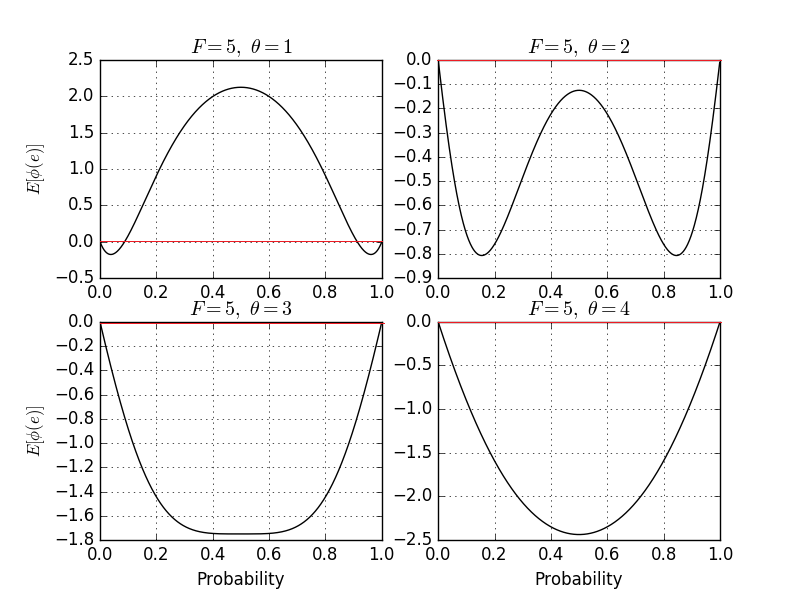
\includegraphics[width=0.5\linewidth]{c:/users/alexander/graphics/F5weight.PNG}
\end{figure}

\clearpage

Some basic properties of $E\phi(e): [0,1] \rightarrow \mathbb{R}$:
\begin{itemize}
\item $E\phi(e)$is continuous differentiable in $p$.
\item $E\phi(e)(p)=0$ for $p\in\{0,1\}$.
\item\ $\frac{dE\phi(e)}{dp} = \sum_{j \leq \theta}(-j)\frac{d}{dp} p_j + \sum_{j>\theta}(j+2(1-\frac{j}{F}))\frac{d}{dp} p_j$ where 
\begin{equation}
\begin{split}
\frac{d}{dp} p_j &= \frac{d}{dp}\binom{F}{j}(2p(1-p))^j(p^2 + (1-p)^2)^{F-j} \\
&= \binom{F}{j}j(2p(1-p))^{j-1}(2-4p)(p^2 + (1-p)^2)^{F - j}\\
& + \binom{F}{j}(2p(1-p))^j(F - j)(4p - 2)(p^2 + (1-p)^2)^{F - j-1} 
\end{split}
\end{equation}
\item $\frac{dE\phi(e)}{dp}(0)=-2F$ and $\frac{dE\phi(e)}{dp}(1)=2F$
\item Symmetry: $E\phi(e)(p)=E\phi(e)(1-p)$. This follows from the symmetry of $p_j = \binom{F}{j}(2p(1-p))^j(p^2+(1-p)^2)^{F-j}$
\item $E\phi(e) \leq 0$ for $F \leq 2\theta-1$. 
\end{itemize}
\clearpage

\textbf{Results:}\\
\mybox{0.8\textwidth}{ 
\textbf{(1)}There exists an open interval $(a,1-a) \subset [0,1]$ such that the system with $F \geq 4\theta $ fixates when started from a product measure with density $p \in (a,1-a)$.
}
\mybox{0.8\textwidth}{ 
\textbf{(2)}There exists an open interval $(a,1-a) \subset [0,1]$ such that the system with $F = 4\theta-1 $ fixates when started from a product measure with density $p \in (a,1-a)$.
}
\mybox{0.8\textwidth}{ 
\textbf{(3)}There exists an open interval $(a,1-a) \subset [0,1]$ such that the system with $F = 4\theta-n $. where $n \in \mathbb{N}$ and $n \leq \min\{\theta-1,2\theta\}$, fixates when started from a product measure with density $p \in (a,1-a)$. 
}
\clearpage

\begin{figure}[!tbp]
  \centering
  \begin{minipage}[b]{0.4\textwidth}
    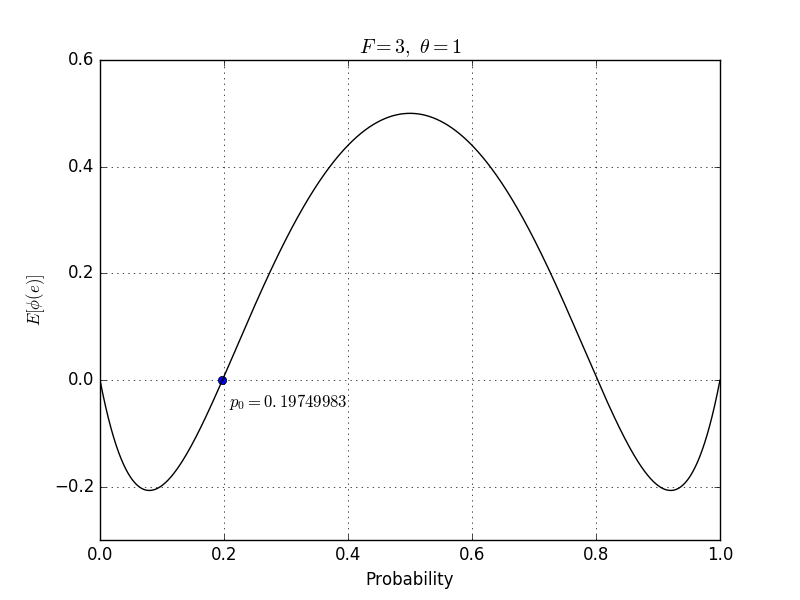
\includegraphics[width=\textwidth]{c:/users/alexander/graphics/F3T1weight.PNG}
  \end{minipage}
  \begin{minipage}[b]{0.4\textwidth}
    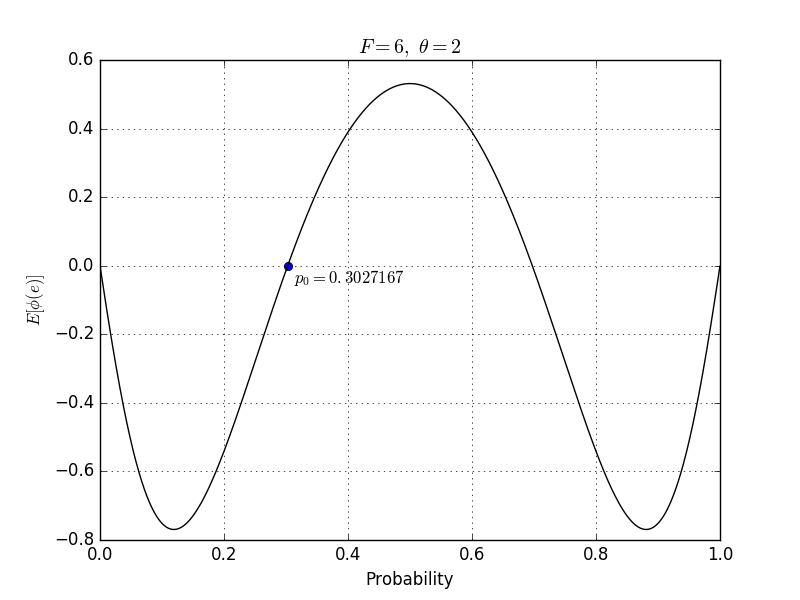
\includegraphics[width=\textwidth]{c:/users/alexander/graphics/F6T2weight.PNG}
  \end{minipage}
    \centering
  \begin{minipage}[b]{0.4\textwidth}
    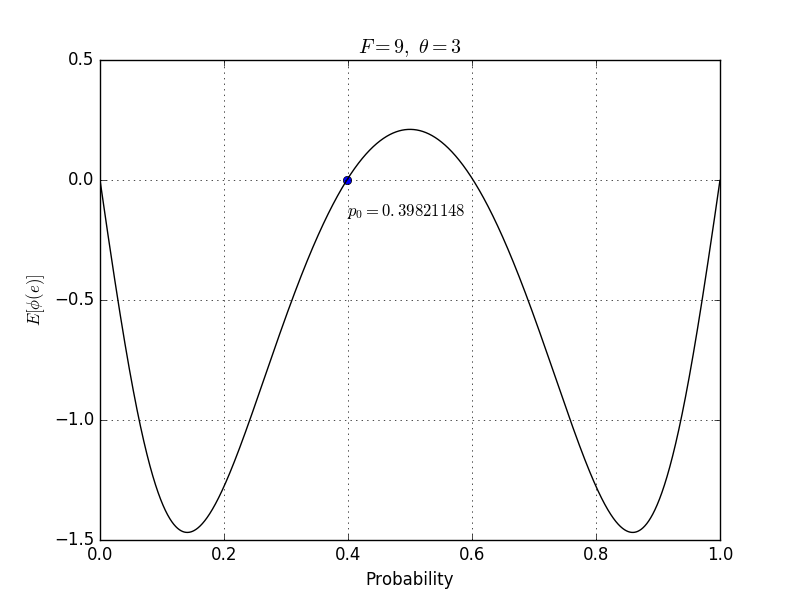
\includegraphics[width=\textwidth]{c:/users/alexander/graphics/F9T3weight.PNG}
  \end{minipage}
  \begin{minipage}[b]{0.4\textwidth}
    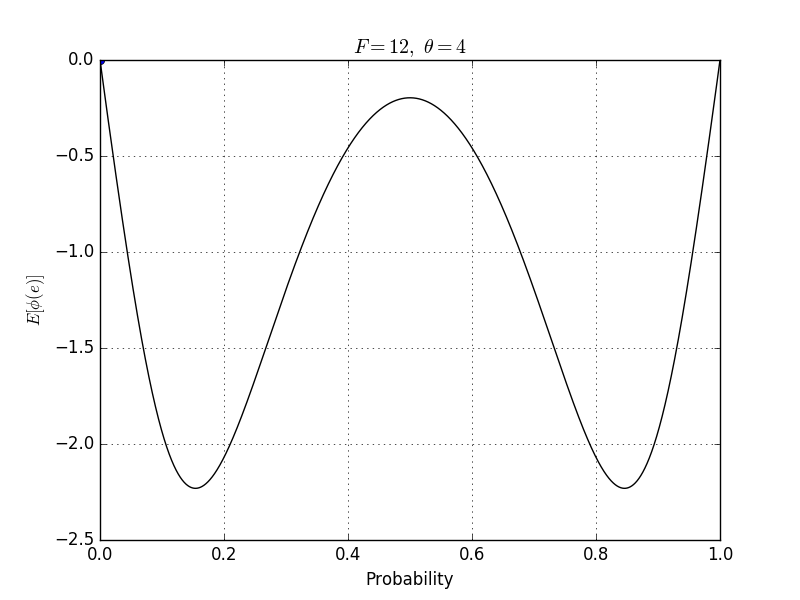
\includegraphics[width=\textwidth]{c:/users/alexander/graphics/F12T4weight.PNG}
  \end{minipage}
\end{figure}

\clearpage

\section{Simulation on Torus}

\ihead{
\hspace{-2mm}
\begin{tikzpicture}[remember picture,overlay]
\node [xshift=\paperwidth/2,yshift=-\headheight] (mybar) at (current page.north west)[rectangle,fill,inner sep=0pt,minimum width=\paperwidth,minimum height=2\headheight,top color=mygreen!64,bottom color=mygreen]{}; % Colored bar
\node[below of=mybar,yshift=3.3mm,rectangle,shade,inner sep=0pt,minimum width=128mm,minimum height =1.5mm,top color=black!50,bottom color=white]{}; % Shadow under the colored bar
shadow
\end{tikzpicture}
\color{white}Simulation}

\begin{itemize}
\item \textbf{Regions:} contiguous sites with the same configuration
\item \textbf{Zones:} contiguous sites with compatible configuration, i.e. no blockades
\item \textbf{Disagreements:} blocked edges 
\end{itemize}

\clearpage

\begin{figure}[!tbp]
  \centering
  \begin{minipage}[b]{0.4\textwidth}
    
\includegraphics[width=\textwidth]{c:/users/alexander/graphics/vDF4T2init.PNG}
    \caption{Initial configuration: F=4, $\theta=2$, $100\times 100$ torus}
  \end{minipage}
  \hfill
  \begin{minipage}[b]{0.4\textwidth}
    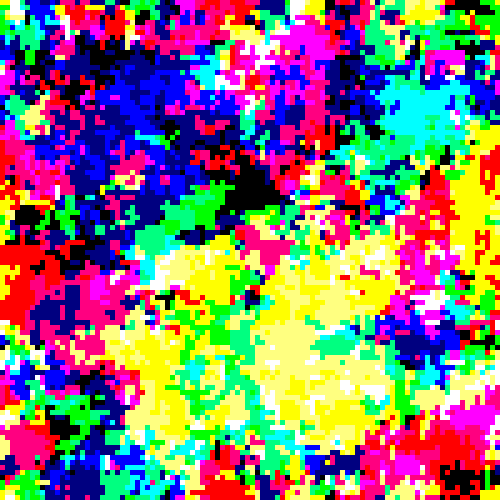
\includegraphics[width=\textwidth]{c:/users/alexander/graphics/vDF4T2_10mil.PNG}
    \caption{10 million successful interactions later}
  \end{minipage}
\end{figure}

\clearpage

\begin{figure}[!tbp]
  \centering
  \begin{minipage}[b]{0.50\textwidth}
    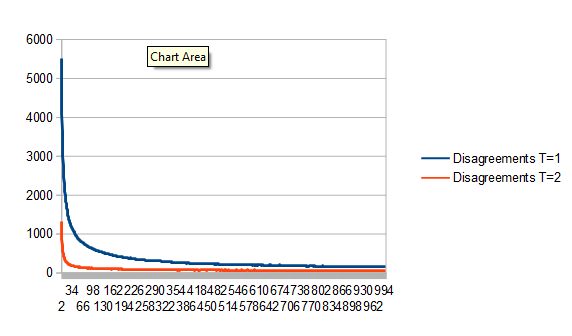
\includegraphics[width=\textwidth]{c:/users/alexander/graphics/F3disagreements.PNG}
  \end{minipage}
  \begin{minipage}[b]{0.50\textwidth}
    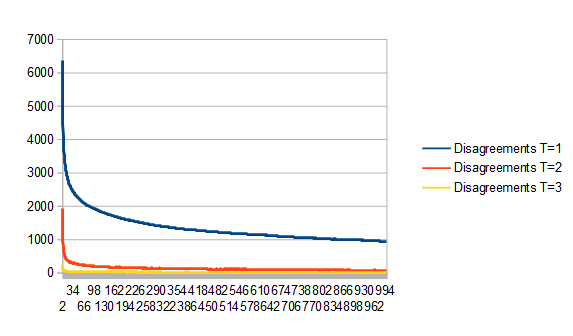
\includegraphics[width=\textwidth]{c:/users/alexander/graphics/F4disagreements.PNG}
  \end{minipage}
\end{figure}

\clearpage

\begin{figure}[!tbp]
  \centering
  \begin{minipage}[b]{0.50\textwidth}
    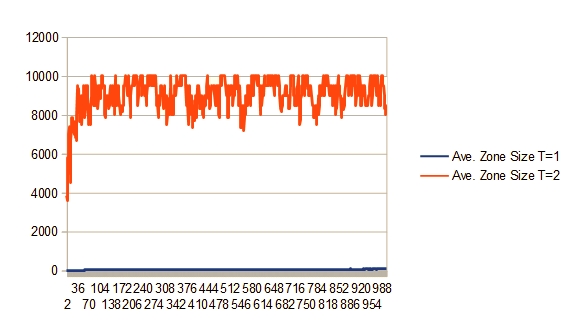
\includegraphics[width=\textwidth]{c:/users/alexander/graphics/F3zones.PNG}
  \end{minipage}
  \begin{minipage}[b]{0.50\textwidth}
    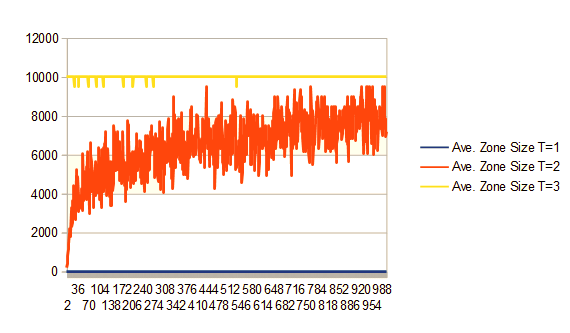
\includegraphics[width=\textwidth]{c:/users/alexander/graphics/F4zones.PNG}
  \end{minipage}
\end{figure}

\clearpage

\begin{figure}[!tbp]
  \centering
  \begin{minipage}[b]{0.50\textwidth}
    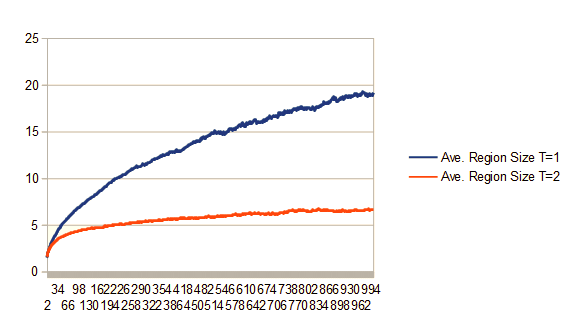
\includegraphics[width=\textwidth]{c:/users/alexander/graphics/F3regions.PNG}
  \end{minipage}
  \begin{minipage}[b]{0.50\textwidth}
    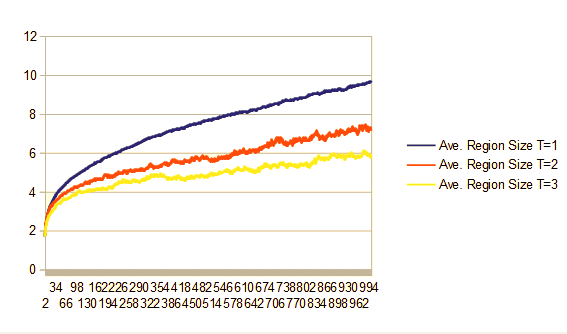
\includegraphics[width=\textwidth]{c:/users/alexander/graphics/F4regions.PNG}
  \end{minipage}
\end{figure}

\clearpage


\begin{thebibliography}{5}

\bibitem{Griffeath81} M. Bramson and D. Griffeath, \emph{On the Williams-Bjerknes Tumour Growth Model I}, Ann. Probab. 9 (2), 173-185 (1981)

\bibitem{Griffeath89} M. Bramson and D. Griffeath, \emph{Flux and Fixation in cyclic particle systems. }, Ann. Probab. 17 (1), 26-45 (1989)

\bibitem{Cox} J.T. Cox and D. Griffeath, \emph{Occupation time limit theorems for the voter model.}, Ann. Probab. 11, 876-893 (1983)

\bibitem{Deffuant et al.} G. Deffuant, D. Neau, F.Amblard and G. Weisbuch, \emph{Mixing beliefs among interacting agents.}, Adv. Compl. Sys. 3, 87-98 (2000)

\bibitem{Harris} T.E. Harris, \emph{Nearest-neighbor Markov interaction processes on multidimensionsional lattices}, Advances in Math. 9, 66-89 (1972)

\bibitem{AxelrodRevised} N. Lanchier, \emph{The Axelrod Model for the Dissemination of Culture Revised}, Ann. Appl. Probab. 2, 860-880 (2012)

\bibitem{FixAxel} N. Lanchier and S. Scarlatos, \emph{Fixation in the One-dimensional Axelrod Model}, Ann. Appl. Probab. 23 (6), 2538-2559 (2013)

\bibitem{ClustCoex} N. Lanchier and S. Scarlatos, \emph{Clustering and coexistence in the one-dimensional vectorial Deffuant model}, Lat. Am. J. Probab. Math. Stat. 11 (2), 541-564 (2014)

\bibitem{FluxvsFix} N. Lanchier and S. Scarlatos, \emph{Fluctuation versus fixation in the one-dimensional constrained voter model}, ArXiv Mathematics e-prints (2014)


\end{thebibliography}
\clearpage

%------------------------------------------------

\thispagestyle{empty} % No slide header and footer

\begin{tikzpicture}[remember picture,overlay] % Background box
\node [xshift=\paperwidth/2,yshift=\paperheight/2] at (current page.south west)[rectangle,fill,inner sep=0pt,minimum width=\paperwidth,minimum height=\paperheight/3,top color=mygreen,bottom color=mygreen]{}; % Change the height of the box, its colors and position on the page here
\end{tikzpicture}
% Text within the box
\begin{flushright}
\vspace{0.6cm}
\color{white}\sffamily
{\bfseries\LARGE Questions?\par} % Request for questions text
\vfill
\end{flushright}

%----------------------------------------------------------------------------------------

\end{document}
